\documentclass{article}
% if you need to pass options to natbib, use, e.g.:
%     \PassOptionsToPackage{numbers, compress}{natbib}
% before loading neurips_2023

% % ready for submission
% \usepackage{neurips_2023}


% to compile a preprint version, e.g., for submission to arXiv, add add the
% [preprint] option:
  % \usepackage[preprint]{neurips_2023}


% to compile a camera-ready version, add the [final] option, e.g.:
    \usepackage[final]{neurips_2023}


% to avoid loading the natbib package, add option nonatbib:
%    \usepackage[nonatbib]{neurips_2023}


\usepackage[utf8]{inputenc} % allow utf-8 input
\usepackage[T1]{fontenc}    % use 8-bit T1 fonts
\usepackage{hyperref}       % hyperlinks
\usepackage{url}            % simple URL typesetting
\usepackage{booktabs}       % professional-quality tables
\usepackage{amsfonts}       % blackboard math symbols
\usepackage{nicefrac}       % compact symbols for 1/2, etc.
\usepackage{microtype}      % microtypography
\usepackage{xcolor}         % colors
\usepackage{multirow}

\usepackage{algorithm}
\usepackage{algpseudocode}
\usepackage{graphicx}
\usepackage{subcaption}
\usepackage{bbm}

\bibliographystyle{unsrtnat}

\title{Causal Effects Under Interference: A Markov Random Field Approach}


% The \author macro works with any number of authors. There are two commands
% used to separate the names and addresses of multiple authors: \And and \AND.
%
% Using \And between authors leaves it to LaTeX to determine where to break the
% lines. Using \AND forces a line break at that point. So, if LaTeX puts 3 of 4
% authors names on the first line, and the last on the second line, try using
% \AND instead of \And before the third author name.


\author{%
  Calvin Walker \\
  % \thanks{Use footnote for providing further information
  %   about author (webpage, alternative address)---\emph{not} for acknowledging
  %   funding agencies.} \\
  % Department of Computer Science\\
  University of Chicago\\
  % Pittsburgh, PA 15213 \\
  \texttt{cswalker1@uchicago.edu} \\
  % examples of more authors
  % \And
  % Coauthor \\
  % Affiliation \\
  % Address \\
  % \texttt{email} \\
  % \AND
  % Coauthor \\
  % Affiliation \\
  % Address \\
  % \texttt{email} \\
  % \And
  % Coauthor \\
  % Affiliation \\
  % Address \\
  % \texttt{email} \\
  % \And
  % Coauthor \\
  % Affiliation \\
  % Address \\
  % \texttt{email} \\
}


\begin{document}


\maketitle


\begin{abstract}
    In randomized experiments, it is often assumed that the response of a given unit only depends on its own characterisitcs and the treatment to which it is assigned. However, there are numerous situations of interest to researchers 
    where this may not be a plausible assuption, particularly when there is social interaction between individuals in an experiment, and the ability to separately identify the effects of treatment assigment and peer influence have important implications. 
    This paper presents a general framework for reliably identifying and estimating causal effects in experimental settings where there is potential interference between units. The framework consists of 
    (i) learning the potential for interference between connected units, (ii) a probabilistic graphical model for estimating individuals' exposure to treated units, and (iii) methods that make use of estimated exposures to compute causal effects of interest. We then evaluate the performance of the proposed framework on by simulating synthetic experimental data on a variety of real world social networks.
\end{abstract}


\section{Introduction}

Reliable causal inference is central to a variety of disciplines in the natural and social sciences. While the Randomized Control Trial (RCT) has long been a gold standard in terms of 
causal inference, central to it is an assumption in the economic literature first coined by \cite{Rubin} known as SUTVA, or the stable unit treatment value assumption, which states that there is no
interference between units, and no hidden variations of treatment. Essentially, the outcome of each individual does not depend on the treatment assigment of others. When this assumption is violated, 
there are said to be spillover effects. In a large-scale RCT on 61 million Facebook Users in the buildup to the 2020 United States Congressional election, the treatment—sending a message that encouraged users to vote—was 
observed to ``spillover'' to the treated individual's closest Facebook friends (\cite{Bond}). 

A number of recent works have sought to address estimation of both treatment and spillover effects in the presence of SUTVA violations, particularly in the context of an observed social network between individuals. \cite{pmlr-v28-toulis13} seek to estimate spillover effects directly, developing both 
an experimental design using sequential randomization, and a Bayesian procedure that assumes a linear response. Other approaches consist of the researcher specifying an ``exposure mapping'' to categorize individuals, e.g. treated, neighbor of treated, etc. and then use 
inverse probability weighting based on the probability of assignment for each individual \cite{Aronow}. Due to the inherent graphical nature of the problem, this paper seeks to examine how a probabilistic graphical model may be well 
suited to capture interference and spillover effects in a social network. We develop a flexible framework that defines a probabilistic graphical model over the social network, and uses this model to estimate unit level exposure to treated units, 
allowing us to compute causal effects of interest. 

\section{Setting and Assumptions}

We consider the setting of a randomized experiment on a social network of $N$ nodes. The network, $G = (V, E)$, is observed, and may or may not contain node-level covariates or edge strengths. 
Let $\mathbf{Z} = (Z_1, Z_2, \dots ,Z_N)$ be a treatment assigment vector over $N$ units, where $Z_i \in \{0, 1\}$ specifies which of the possible treatments unit $i$ receives. 
We assume that $P(Z_i = 1)$ is the same for all $i \in \{N\}$, so treatment assigment is unconfounded. We define $\mathbf{C} = (C_1, C_2, \dots, C_N)$ to be a latent exposure vector, where $C_i \in \{0, 1\}$ specifies if unit $i$ is exposed to the treatment via social interaction. 
Here, we assume that all treated units are exposed, such that $Z_i \times C_i = 1$, but that treatment units do not experience further spillover effects. %TODO: go more indepth on this 
If we could observe $\mathbf{C}$, then our work would be done, since we could partition the units into treatment, exposure, and control groups, and employ classic techniques to infer their differences in outcome. 

Instead, we define $\pi_i = P(C_i = 1)$ to be the expsoure probability for unit $i$ given some instantiation of the experiment $\mathbf{Z}, \mathbf{C}$. Since an individual's social exposure to the treatment depends on the random assigment in $G$, so does $\pi_i$. For simplicity, we assume that
the effect of treatment assigment is homogeneous. Furthermore, we assume that social interaction, and thus social exposure to the treatment, only occurs through the edges $E$ of $G$. However, we do not assume that spillover effects are homogeneous, and examine both this and the heterogeneous case in later sections.

\section{Estimating Exposures and Causal Effects}

We propose modeling the spread of influence in the social network as a Pairwise Markov Random Field, defined as $B = (P, H)$, where $H = (V, E)$ is an isomorphic to the social network $G$, given by the bijection $f: G(V) \mapsto H(V)$ where $f(v_i) = X_i \sim $ Bernoulli$(p)$, i.e. $H$ is an undirected graph with the skeleton of $G$ where each node in $H(V)$ is a Bernoulli random variable. 
$P$, then, is defined as a Gibbs distribution that factorizes over $H$: \\
\begin{displaymath}
  P(X_1, X_2, \dots, X_n) = \frac{1}{Z}\prod_{i \in V} \phi_i(X_i)\prod_{(i, j) \in E}\phi_{i,j}(X_i, X_j) \\[0.5ex]
\end{displaymath}
By having each individual represented as a Bernoulli random vairable in $H$, we can reformulate the problem of estimating the exposure probability for node $i$,  $\pi_i$, into 
an inference problem where we seek to infer marginal probability distributions for each node. Observe that for any treated unit, they are assumed to be already exposed, so $X_i = 1$ for all individuals $i$ where $Z_i = 1$. 
This observation acts as our evidence in $P$ when performing inference on the unknown marginal distributions of the other nodes in $H$. Formally, we infer the marginal distribution $P(X_i\ |\ e)$, for each $i \in \{N\}$, where $e = \{X_i = 1\ |\ Z_i = 1\}$. 
This reformulation allows us to use a host of existing inference algorithms to learn the marginals. In practice, we define a clique tree $\mathcal{T}$ for $B$, and then use the Sum-Product Belief Propogation algorithm (CTree-SP-Calibrate) defined in \cite{koller}. 
\begin{algorithm}[h]
  \caption{CTree-SP-Calibrate}
  % \label{algo1}
   \begin{algorithmic}[1]
       \Require $\Phi, \mathcal{T}$
       \State Initialize Cliques
       \While{$\exists \ i, j$ such that $i$ is ready to transmit to $j$}
       \State $\psi(\mathcal{C}_i) \leftarrow \psi_i \cdot \prod_{k \in Nb(i) - j}m_{k \rightarrow i}$
       \State $m_{i \rightarrow j}(S_{i,j}) \leftarrow \sum_{\mathcal{C}_i - S_{i,j}}\psi(\mathcal{C}_i)$
       \EndWhile
       \For{each clique $i$}
       \State $\beta_i \leftarrow \psi_i \cdot \prod_{k \in Nb(i) - j}m_{k \rightarrow i}$
       \EndFor \\

       \Return $\{\beta_i\}$
\end{algorithmic}
\end{algorithm}
In larger social networks where exact inference may be intractable, 
approximation alogrithms can be used, although we do not examine this case. Since nodes not influenced by the treatment group have the marginal distribution: $P(X_i = 1) = P(X_i = 0) = 0.5$, we let $\pi_i = P(X_i = 1) - P(X_i = 0)$ to obtain easily interpretable exposure probabilities on the interval $[0, 1]$.
%Algorithm 1: Sum-Product BP 



% In the case of larger social networks where exact inference may be intractable, approximation 
% algorithms can be used, although this paper does not  

% discuss posterior marginals --> exposure probabilities 

\subsection{Unary and Edge Potentials}

Having refomulated estimating $\pi_i(\mathbf{Z})$ as inference of marginals in a Pairwise MRF, 
properly defining the edge and unary potentials in $H$ becomes an important specification. In this section, 
we dicuss several potential approaches. In the setting considered by this paper, treatment assigment is unconfounded, so 
the unary potentials $\phi_i(X_i)$, are uniform across the nodes such that $\phi_i(X_i = 1) = \phi_i(X_i = 0) \ \forall i$. However, 
in the case that treatment assigment is, for instance, confounded by covariates, it may make sense to use the unary potentials as a prior on similarity 
with the treatment group, since influence may flow to ``similar'' nodes more easily. 

The edge potentials $\phi_i(X_i, X_j)$ have an even more intuitive interpretation, representing the potential for influence, or ``strength'' of a social connection between two nodes in $H$. Here, 
we propose two possible approaches for specifying the edge potentials. Both involve first specifying the probability of each edge in the social network. The first is that, given domain knowledge within the experiment, the researcher may have a prior on the distribution of 
edge probabilities, and can make use of this prior belief. For instance, let $p_{i,j}$ be the probability of an edge between node 
$i$ and node $j$. A reasonable prior could be $p_{i,j} \sim $ Beta$(5, 5)$. This belief could be incorporated by initializing the 
edge potentials according to this distribution. The next is a latent variable model introduced by \cite{Handcock}. Where we model $p_{i,j}$ using a logistic regression where the probability of an edge depends on euclidean distance in latent space: 
\begin{equation}
  \mbox{log-odds}(p_{i,j}) = \beta X_{i,j} - |z_i - z_j|
\end{equation}
Where $z_i$ and $z_j$ are node $i$ and node $j$'s respective positions in latent space, and $X_{i,j}$ is some vector valued edge covariates. Here, it is assumed that the existence of an edge is independent of other edges. 
Handcock jointly estimates the parameter $\beta$ and the latent $z_i$'s using MCMC, with prior: \begin{displaymath}
  z_i \sim \sum_{g = 1}^{G}\lambda_g \mbox{MVN}_d(\mu_g, \sigma_gI_g) 
\end{displaymath}
Where $G$ is the possible number of latent social clusters. Since we can take $G = 1$, the latent variable model provides a flexible and well 
studied approach to estimating the probability of edges between nodes in a variety of experimental settings. We test both possible approaches to estimating 
edge probabilities in the following section.
%more discussion 

%figure Beta(5, 5) vs empirical distribution of latent probabilities. 
Given the edge probabilities $p_{i,j}$, we can specify the the edge potentials in $H$. In doing so, 
we make the assumption that a higher edge probability leads to greater social influence, and thus likelihood that two adjacent nodes 
have the same value, i.e. $P(X_i = X_j)$ is monotonically increacing in $p_{i,j}$. To acheive this, we define the edge potentials as:
\begin{displaymath}
  \phi_{i,j}(X_i, X_j) = 1 - p_{i,j}\mathbbm{1}\{{X_i \neq X_j}\} \\[0.5ex]
\end{displaymath}
We found that this specification resulted in a plausible empirical results across a number of different social networks, but this is another place where a researcher may choose to 
incorporate prior beliefs in specifying how social influence propogates in a specific network.

\subsection{Estimating Causal Effects}

With a distribution over the exposure probabilities for each node, we can turn to the problem of estimating the causal effects of interest. 
First, we are interested in estimating the average treatment effect, ATE. A naïve estimate of ATE in our setting would be a simple difference of means 
between the treatment and control groups. However, as discussed, in the presence of spillover effects, this estimate is that of both ATE, and whatever spillover 
effects may be present in the experiment. Instead, we propose the OLS regression: 
\begin{equation}
  y_i = \alpha + \rho Z_i + \gamma (1 - Z_i) \pi_i + \varepsilon_i \\[1.0ex]
\end{equation}
Where $\rho$ is the parameter of interest. Since $\pi_i = 1$ if $Z_i = 1$, we add the interaction term $(1 - Z_i)$, so that the causal effect of
treatment assigment is only contained in $\rho$. Unfortunatley, the coefficient $\gamma$ does not have much causal interpretation, since $\pi_i$ is merely the probability that unit $i$
is socially exposed to the treatment. In theory, the above regression model, and our approach in general, is better suited to the heterogeneous spillover effects case, since potential outcomes are linear in $\pi_i$. 
In this case, we could interperent $\gamma \times \pi_i$ to be the partial effect of exposure for unit $i$. 

In the case of homogeneous spillover effects, what we really desire is to be able to classify each non-treated unit into either the socially exposed ($C_i = 1$), or control group $(C_i = 0)$, as doing so 
would allow for perfect identification of average spillover effects. There are a number of possible approaches. One might be assigning units with exposure probability sufficiently close to zero to the control group, 
and having a similar condition for assigment to the expsoure group. Another may be to explicitly learn a classifier. If treatment assigment were confounded by latent or observed covariates, this may be possible without 
taking the outcome of interest into account, since the treatment and exposure groups would have greater similarity than the controls. However, the setting of this paper assumes that treatment assigment is unconfounded. Under 
the assumption that the joint distribution of outcomes and exposures, $P(y, \pi)$ is a mixture of two Gaussians—the control and exposure groups—we propose fitting the Gaussian Mixture Model: \begin{equation}
  P(y, \pi | \mu, \Sigma, w) = \sum_{k = 1}^{2}w_k \mathcal{N}(y, \pi ; \mu_k, \Sigma_k)
\end{equation} 
And then estimating the average spillover effect as the difference in means: $\bar{y}^{k = 2} - \bar{y}^{k = 1}$, where $k \in \{1, 2\}$ indexes the control and expsoure groups, respectively.

\section{Simulations}

In order to test the performance of our proposed methods, we simulate random experiments on two real world social networks. The first is a group of 55 eigth-graders, with edges between 
students who were surveyed on which other students they would like to sit next to in class. The second data set is a social network between 61 employees of the Aarhus Computer Science Department, where 
edges represent colleagues who ate lunch together in a given week. We simlulate the outcome of interest drawing from a normal distribution $y_{i} \sim \mathcal{N}(\mu, \sigma^2)$, and then consider a dilated effects scenario, 
where spillover is half of the average treatment effect. For each graph, we consider three possible data generating processes for the spillover effects, and a fourth where there are no spillover effects. In the first, all neighbors of treated units are socially influenced. 
In the second, social influence is propogated across each edge $(i, j)$ with probability $p_{i,j}$ according to the latent variable model (1), i.e. socially influenced neighbors of treated units can influence their neighbors etc. until all possible influence
has propogated across the network. The third is the same as the second process except $p_{i,j} = 0.5$ for all edges in the network. We also test two different spesifications for the edge potentials in each scenario. In the first, the edge potentials accord with the latent variable model (1), and in the second we assume that $p_{i,j} \sim$ Beta$(5, 5)$. The following table report the point estimates of the OLS regression (2) and corresponding standard errors following 1,000 simulated 
treatment assigments on each of the possible combinations of data generating processes, edge potentials, and social networks. 
\begin{table}[htbp]
  \caption{Simulation Results (True parameter: $\rho = 3$)}
  \label{table1}
  \centering
  \begin{tabular}{ccccccc}
    \toprule
    & & \multicolumn{2}{c}{Eighth Graders} & & \multicolumn{2}{c}{Aarhus CS}              \\
    \cmidrule{3-4} \cmidrule{6-7}
    DGP & $\phi_{i,j}$ & $\bar{y}^1 - \bar{y}^0$ & $\rho$ & & $\bar{y}^1 - \bar{y}^0$ & $\rho$ \\
    \midrule
    \multirow{ 2}{*}{Neighbors} & Latent & 2.67 (0.22) & 3.03 (0.30) & & 2.31 (0.21) & 3.03 (0.43)    \\
    \cmidrule{2-7}
    & Beta & 2.66 (0.22) & 3.14 (0.38) & & 2.32 (0.21) & 3.63 (0.63)  \\
    \midrule
    \multirow{ 2}{*}{Latent}& Latent & 2.73 (0.22) & 2.93 (0.33)  & & 2.55 (0.21) & 2.93 (0.43)  \\
    \cmidrule{2-7}
    & Beta  & 2.72 (0.22) & 2.95 (0.35)  & & 2.54 (0.21) & 3.08 (0.61) \\
    \midrule
    \multirow{ 2}{*}{$p_{i,j} = 0.5$}& Latent & 2.55 (0.22) & 2.67 (0.38)  & & 2.31 (0.21) & 2.48 (0.46) \\
    \cmidrule{2-7} 
    & Beta  & 2.56 (0.23)& 2.81 (0.40)  & & 2.32 (0.21) & 2.64 (0.67)  \\
    \midrule
    \multirow{ 2}{*}{No Spillover}& Latent & 3.00 (0.21) & 3.00 (0.24)  & & 3.01 (0.19) & 3.01 (0.27) \\
    \cmidrule{2-7} 
    & Beta  & 3.00 (0.20) & 3.00 (0.25)  & & 2.99 (0.19) & 2.99 (0.38)  \\
    \bottomrule
  \end{tabular}
\end{table}

In general, the point estimates for $\rho$ are an improvement over the naïve estimate $\bar{y}^{1} - \bar{y}^{0}$. However, 
performance was quite varied across the different data generating processes. In particular, the model was not well suited to capture the effects of the third DGP ($p_{i,j} = 0.5$), even in the 
case of the Beta prior on the edge potentials, which had quite high Standard Errors for the Aarhus Computer Science dataset. Still, in the first two data generating processes, 
which are quite different from one another, our model is able to reliably detect the presence, and extent of spillover effects in the data, isolating the average treatment effect as desired. Furthermore, 
in the case of no spillover effects, we still get the correct point estimate, demonstrating the usefulness of our framework. Next, we test performance when spillover effects are heterogeneous, which is the natural setting for our model. In the following table, we report results from an identical simulation as above, instead 
now spillover effects are propogated across each edge $(i-j)$ proportional to $p_{i,j}$ according to the latent variable model (1). We do this by conducting a breadth first traversal over the graph where 
the starting queue is the treatment group. 
\begin{table}[htbp]
  \caption{Heterogeneous Spillover Effects Simulation Results (True parameter: $\rho = 3$)}
  \label{table2}
  \centering
  \begin{tabular}{cccccccc}
    \toprule
    & \multicolumn{3}{c}{Eighth Graders} & & \multicolumn{3}{c}{Aarhus CS}              \\
    \cmidrule{2-4} \cmidrule{6-8}
    $\phi_{i,j}$ & $\bar{y}^1 - \bar{y}^0$ & $\rho$ & $\gamma$ & & $\bar{y}^1 - \bar{y}^0$ & $\rho$ & $\gamma$ \\
    \midrule
     Latent & 2.74 (0.21) & 2.95 (0.25) & 1.40 (0.39) & & 2.64 (0.20) & 2.99 (0.31) & 0.48 (0.25)    \\
    \cmidrule{1-8}
    Beta & 2.75 (0.21) & 2.99 (0.28) & 0.84 (0.40) & & 2.65 (0.20) & 3.06 (0.38) & 0.51 (0.36) \\
    \bottomrule
  \end{tabular}
\end{table}

As expected, when the underlying data generating process consists of heterogeneous spillover effects, the model performs better, particularly with respect 
to standard error, which is quite high in the homogeneous case. Somewhat surprisingly, the Beta prior performs decently well on both graphs, despite the spillover 
effects propogating accoring to the latent variable model. 

Finally, we test the proposed Gaussian Mixure Model (3) using two of the previous data generating processes. We 
use the latent variable model (1) to determine edge potentials. Below, Figure 1 displays the fitted GMMs. The 
corresponding point estimates for the average spillover effect were $1.67$ (DGP $p_{i,j} = 0.5$) and $1.61$ (DGP Neighbors), where $1.5$ is the value of the true parameter. 

\begin{figure}[htbp]
  \centering
  \begin{subfigure}[b]{0.45\textwidth}
      \centering
      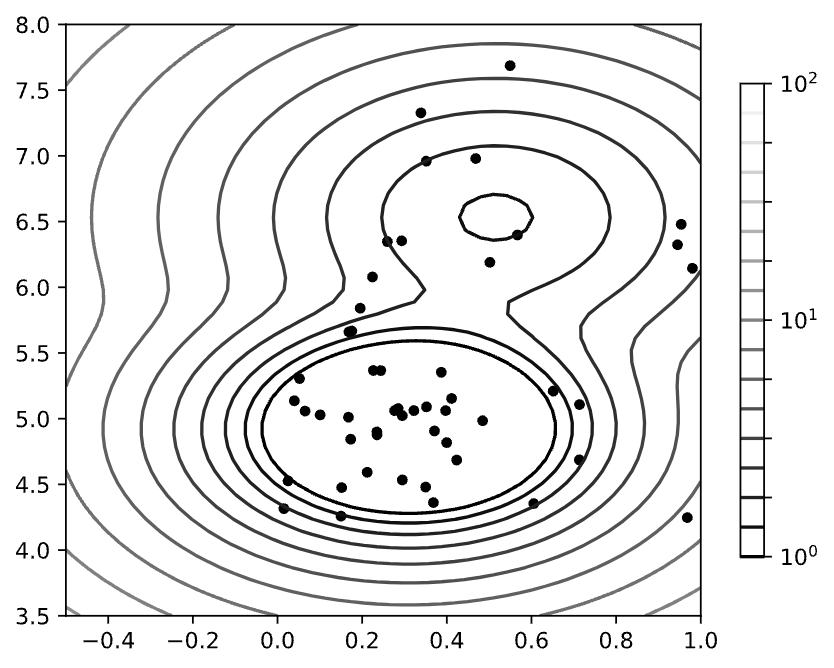
\includegraphics[width=\textwidth]{gmmpij.png}
      \caption{$p_{ij} = 0.5$}
      \label{fig:fig1}
      \vspace{0.25cm}
  \end{subfigure}
  \hfill
  \begin{subfigure}[b]{0.45\textwidth}
      \centering
      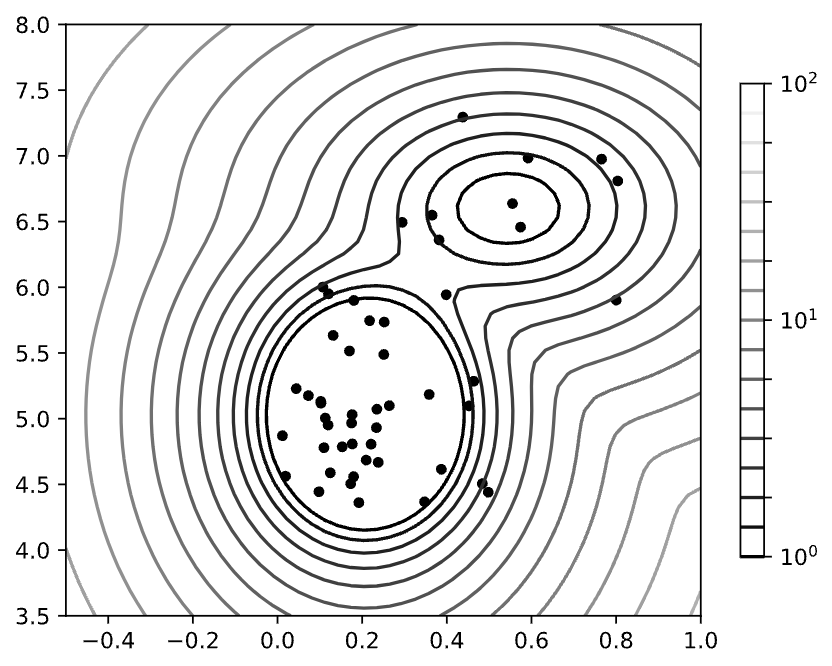
\includegraphics[width=\textwidth]{gmmnbrs.png}
      \caption{Neighbors}
      \label{fig:fig2}
      \vspace{0.25cm}
  \end{subfigure}
  \caption{Gaussian Mixture Model Negative Log Likelihood (X-axis: $\pi$, Y-axis: $y$)}
  \label{fig:side_by_side}
\end{figure}

While the GMM produces reasonable estimates for the average spillover effects, it does require imposing potentially undesireable assumptions, in 
addition to using knowledge of unit-level outcomes. For these reasons, it is unlikely to generalize well to other experimental settings.   

\section{Conclusion}

This paper proposes a probabilistic graphical model based framework for causal inference under interference in social networks. In particular, 
we define a pairwise Markov Random Field over the social network, that allows us to infer exposure probabilities given a particular instantiation of the 
random experiment. We examine the performance of the proposed framework in a variety of plausible settings and data generating processes for spillover effects,
and find that it can reliably detect the presence, or non-presence, of spillover. While the Markov Random Field approach is well suited to estimating the average treatment effect, 
more research is necessary to develop reliable and flexible estimators that extend this framework to estimate the spillover effects directly, particularly in the case of homogeneous 
spillover. 





\bibliography{rep}


% {
% \small



% [1] Handcock, M.S., Raftery, A.E. and Tantrum, J.M. (2007), Model-based clustering for social networks. Journal of the Royal Statistical Society: Series A (Statistics in Society), 170: 301-354. https://doi.org/10.1111/j.1467-985X.2007.00471.x


% % [1] Alexander, J.A.\ \& Mozer, M.C.\ (1995) Template-based algorithms for
% % connectionist rule extraction. In G.\ Tesauro, D.S.\ Touretzky and T.K.\ Leen
% % (eds.), {\it Advances in Neural Information Processing Systems 7},
% % pp.\ 609--616. Cambridge, MA: MIT Press.


% % [2] Bower, J.M.\ \& Beeman, D.\ (1995) {\it The Book of GENESIS: Exploring
% %   Realistic Neural Models with the GEneral NEural SImulation System.}  New York:
% % TELOS/Springer--Verlag.


% % [3] Hasselmo, M.E., Schnell, E.\ \& Barkai, E.\ (1995) Dynamics of learning and
% % recall at excitatory recurrent synapses and cholinergic modulation in rat
% % hippocampal region CA3. {\it Journal of Neuroscience} {\bf 15}(7):5249-5262.
% }

%%%%%%%%%%%%%%%%%%%%%%%%%%%%%%%%%%%%%%%%%%%%%%%%%%%%%%%%%%%%


\end{document}